\documentclass{beamer}
\usetheme{Madrid}
\usecolortheme{default}


\usepackage[T1]{fontenc}
\usepackage[utf8]{inputenc}
\usepackage{amsmath,amssymb,bm,mathtools}
\usepackage{xcolor}
\usepackage{hyperref}
\usepackage{microtype}

\graphicspath{{./figures/}}
\usepackage{booktabs}


\title[Project 2]{Project 2}
\subtitle{CS 332, Fall 2025}
\author{Ben Cole \and Koshi Harashima}
\date{22 October, 2025}

\begin{document}

\maketitle

\begin{frame}{Outline}
  \tableofcontents
\end{frame}

%===================== we can skip this section! ==========================================
\section{Basic Setting}

\begin{frame}{Basic Setting : Online Learning}
    \textbf{Online Learning}: 
    \begin{itemize}
        \item k actions
        \item n rounds
        \item action $j$'s payoff in round i ; $v_j^i \in [0,h]$
        \item in round i:
        \begin{itemize}
            \item choose an action $j^i$
            \item learn payoffs $v_1^i, \dots, v_k^i$
            \item obtain payoff $v_j^i$
        \item Payoff $ALG = \sum_{i = 1} ^n v_j^i$
        \item the best in hindsight payoff is 
        \[
        OPT = max_j \sum_{i = 1} ^n v_j^i
        \]
        \item the regret of the algorithm is 
        \[
        Regret_n = \frac{1}{n}[OPT - ALG]
        \]
        \end{itemize}   
    \end{itemize}
\end{frame}

\begin{frame}{Basic Setting : EW Algorithm}
    \textbf{Algorithm}\\
    Exponential Weight Algorithm is implemented as follow; 
    \begin{itemize}
        \item learning rate $\epsilon$
        \item let $V_j^i = \sum_{r = 1}^i v_j^i$
        \item in round i choose j with probability $\pi_j^i$ proportional to $(1+\epsilon)^{\frac{V_j^{i-1}}{h}}$
        \item implemented as follow;
        {\small
        \[
            \pi_j^i = \frac{(1+\epsilon)^{\frac{V_j^{i-1}}{h}}}{\sum_{j'}(1+\epsilon)^{\frac{V_{j'}^{i-1}}{h}}}
        \]}
    \end{itemize}
    \textbf{Regret Bound}
    
    

\end{frame}

\begin{frame}{Basic Setting; MC Simulation}
    \textbf{Monte Carlo Simulation}\\
    we implemented MC Simulation as follow;
    \begin{itemize}
        \item fix k, n, tiem(we set 2000 times)
        \item for each times, 
        \begin{enumerate}
            \item set $\epsilon$ to {$0.0001, \sqrt{log\frac{k}{n}}, 10000$}
            \item simulate it through implemented algorithms in each setting.
            \item calculate Regret (total Payoff, and his set of choices)
        \end{enumerate}
        \item then aggregate these results, and calculate mean of Regret and their confident intervals.
    \end{itemize}
    \textbf{learning rates}\\
    \begin{itemize}
      \item No learning: \(\epsilon = 0\) .
      \item Theoretical: \(\epsilon = \sqrt{\ln k / n}\).
      \item FTL:  \(\epsilon \approx \infty\).
    \end{itemize}
\end{frame}

\begin{frame}{Basic Setting : Summary}
    So, Here is a summary. In each part, we show 5 things
    \begin{enumerate}
        \item Game settings
        \item Their structure and our intuition of results
        \item The change of Regret in rounds
        \item The change of total payoffs in rounds
        \item Calculation of Regret bound of optimal learning rate
    \end{enumerate}
    Maybe, we will describe some observations from the analysis of comparative statics(changing parameters). 
\end{frame}
%===================== we can skip this section! ==========================================

\section{Part1}
\begin{frame}{Part1 - Outline}
In Part 1, we consider two things;
\begin{enumerate}
    \item Adversarial Fair Payoffs (AFP) 
    \item Bernoulli Payoffs (BP)
\end{enumerate}
\end{frame}

\begin{frame}{Part1 - Summary}

\textbf{Methods}\\

\textbf{Results}\\

\textbf{Takeaways}\\

\end{frame}

\subsection{A: AFP}

\begin{frame}{A- Setting}
    In each round i:
    \begin{itemize}
        \item Draw a payoff $x \sim U[0,1]$ (i.e., from the uniform distribution on interval [0,1])
        \item Assign this payoff to the action $j^*$ that has the smallest total payoff so far,\\
        i.e., $j^* = \arg\min_j V^{i-1}_{j} \quad \text{where} \quad V^{i}_{j} = \sum_{r=1}^{i} v^{r}_{j}$
        \item (All other actions get 0 payoff in round i.)
    \end{itemize}
    \vspace{1em}
    Here's our parameters;
    \begin{itemize}
        \item k = 
        \item n = 
    \end{itemize}
\end{frame}

\begin{frame}{A - Game structure and Intuition}
    Here's game structure and out intuition is that FTL will work poorly because the more aggressively one seeks to maximize profit, the lower the realized profit due to the fair structure of this game. In addtion, since payoffs are drawn from uniform distribution, we don't predict the cumulative payoff for each arms.
    
    
\end{frame}


\begin{frame}{A - Results(Regret)}
\textbf{Results}\\
Here is a graph showing the change in regret. \\
We conclude that these results are consistent with the intuition.
\begin{center}
    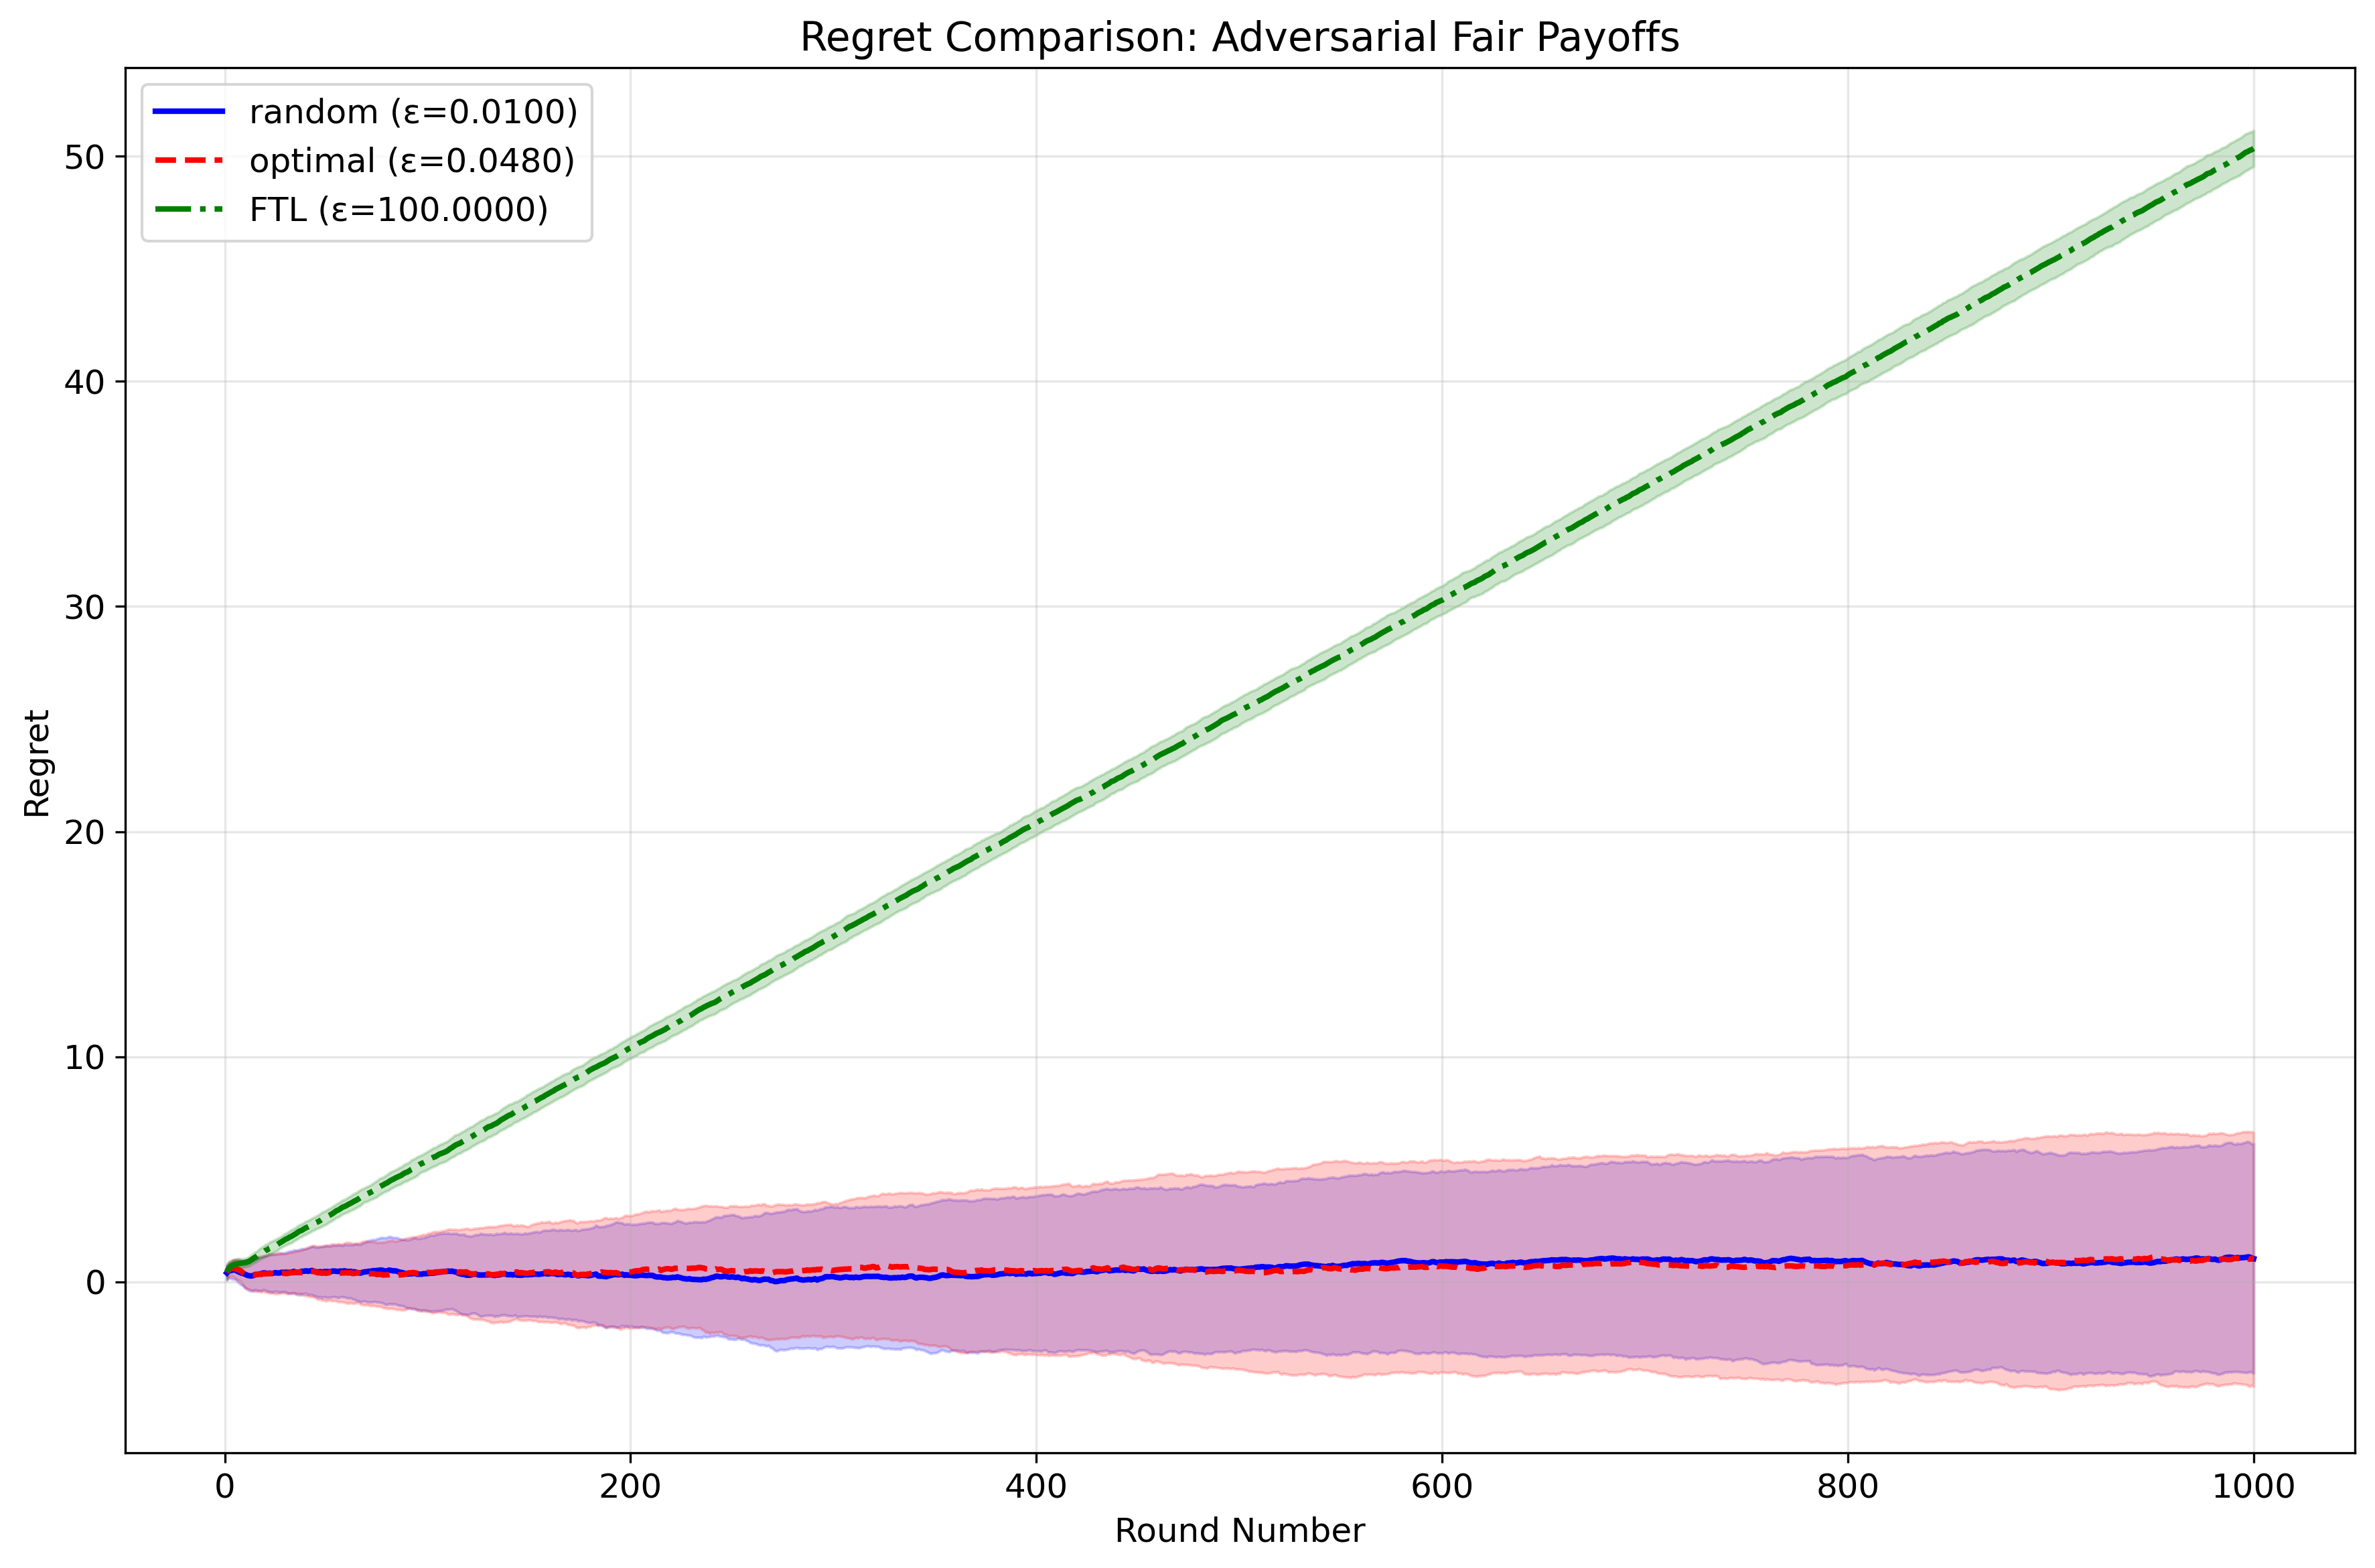
\includegraphics[width=0.7\textwidth]{332Project2/figures/adversarial_regret_comparison.png}
\end{center}
\end{frame}

\begin{frame}{A - Results(Payoffs)}

\end{frame}

\begin{frame}{A - Results(Regret Bound)}
    
\end{frame}

\subsection{B : BP}

\begin{frame}{B - Setting:}
    Fix a probability for each action $p_{1},...,p_{k}$ with each $p_{k}$ in [0,1/2].\\
    In each round i,
    \begin{itemize}
        \item draw the payoff of each action j as $v^{i}_{j} \sim B(p_{j})$ (i.e, from the Bernoulli distribution with probability $p_j$ of being 1 and probability $1-p_{j}$ of being 0).
    \end{itemize}
    \vspace{1em}
    Here's our parameters;
    \begin{itemize}
        \item k = 
        \item n = 
    \end{itemize}
\end{frame}

\begin{frame}{B - Game structure and Intuition}
    Here's game structure and out intuition is that since there are fixed probability, FTL will find the best machine with highest probability while optimal will slowly approaching toward the best machine, random will work poorly.
\end{frame}

\begin{frame}{B - Results(Regret)}
\textbf{Results}\\
Here is a graph showing the change in regret. \\
We conclude that these results are consistent with the intuition. \\
There is the most profitable actions and learning algorithm want to converge to the choices to the one, then randomization deter this optimization, while FTL works pretty good though there's a possiblity of converges to the local optima. But, even if you consider CI, we could say in this setting, FTL preforms best among three.
\begin{center}
    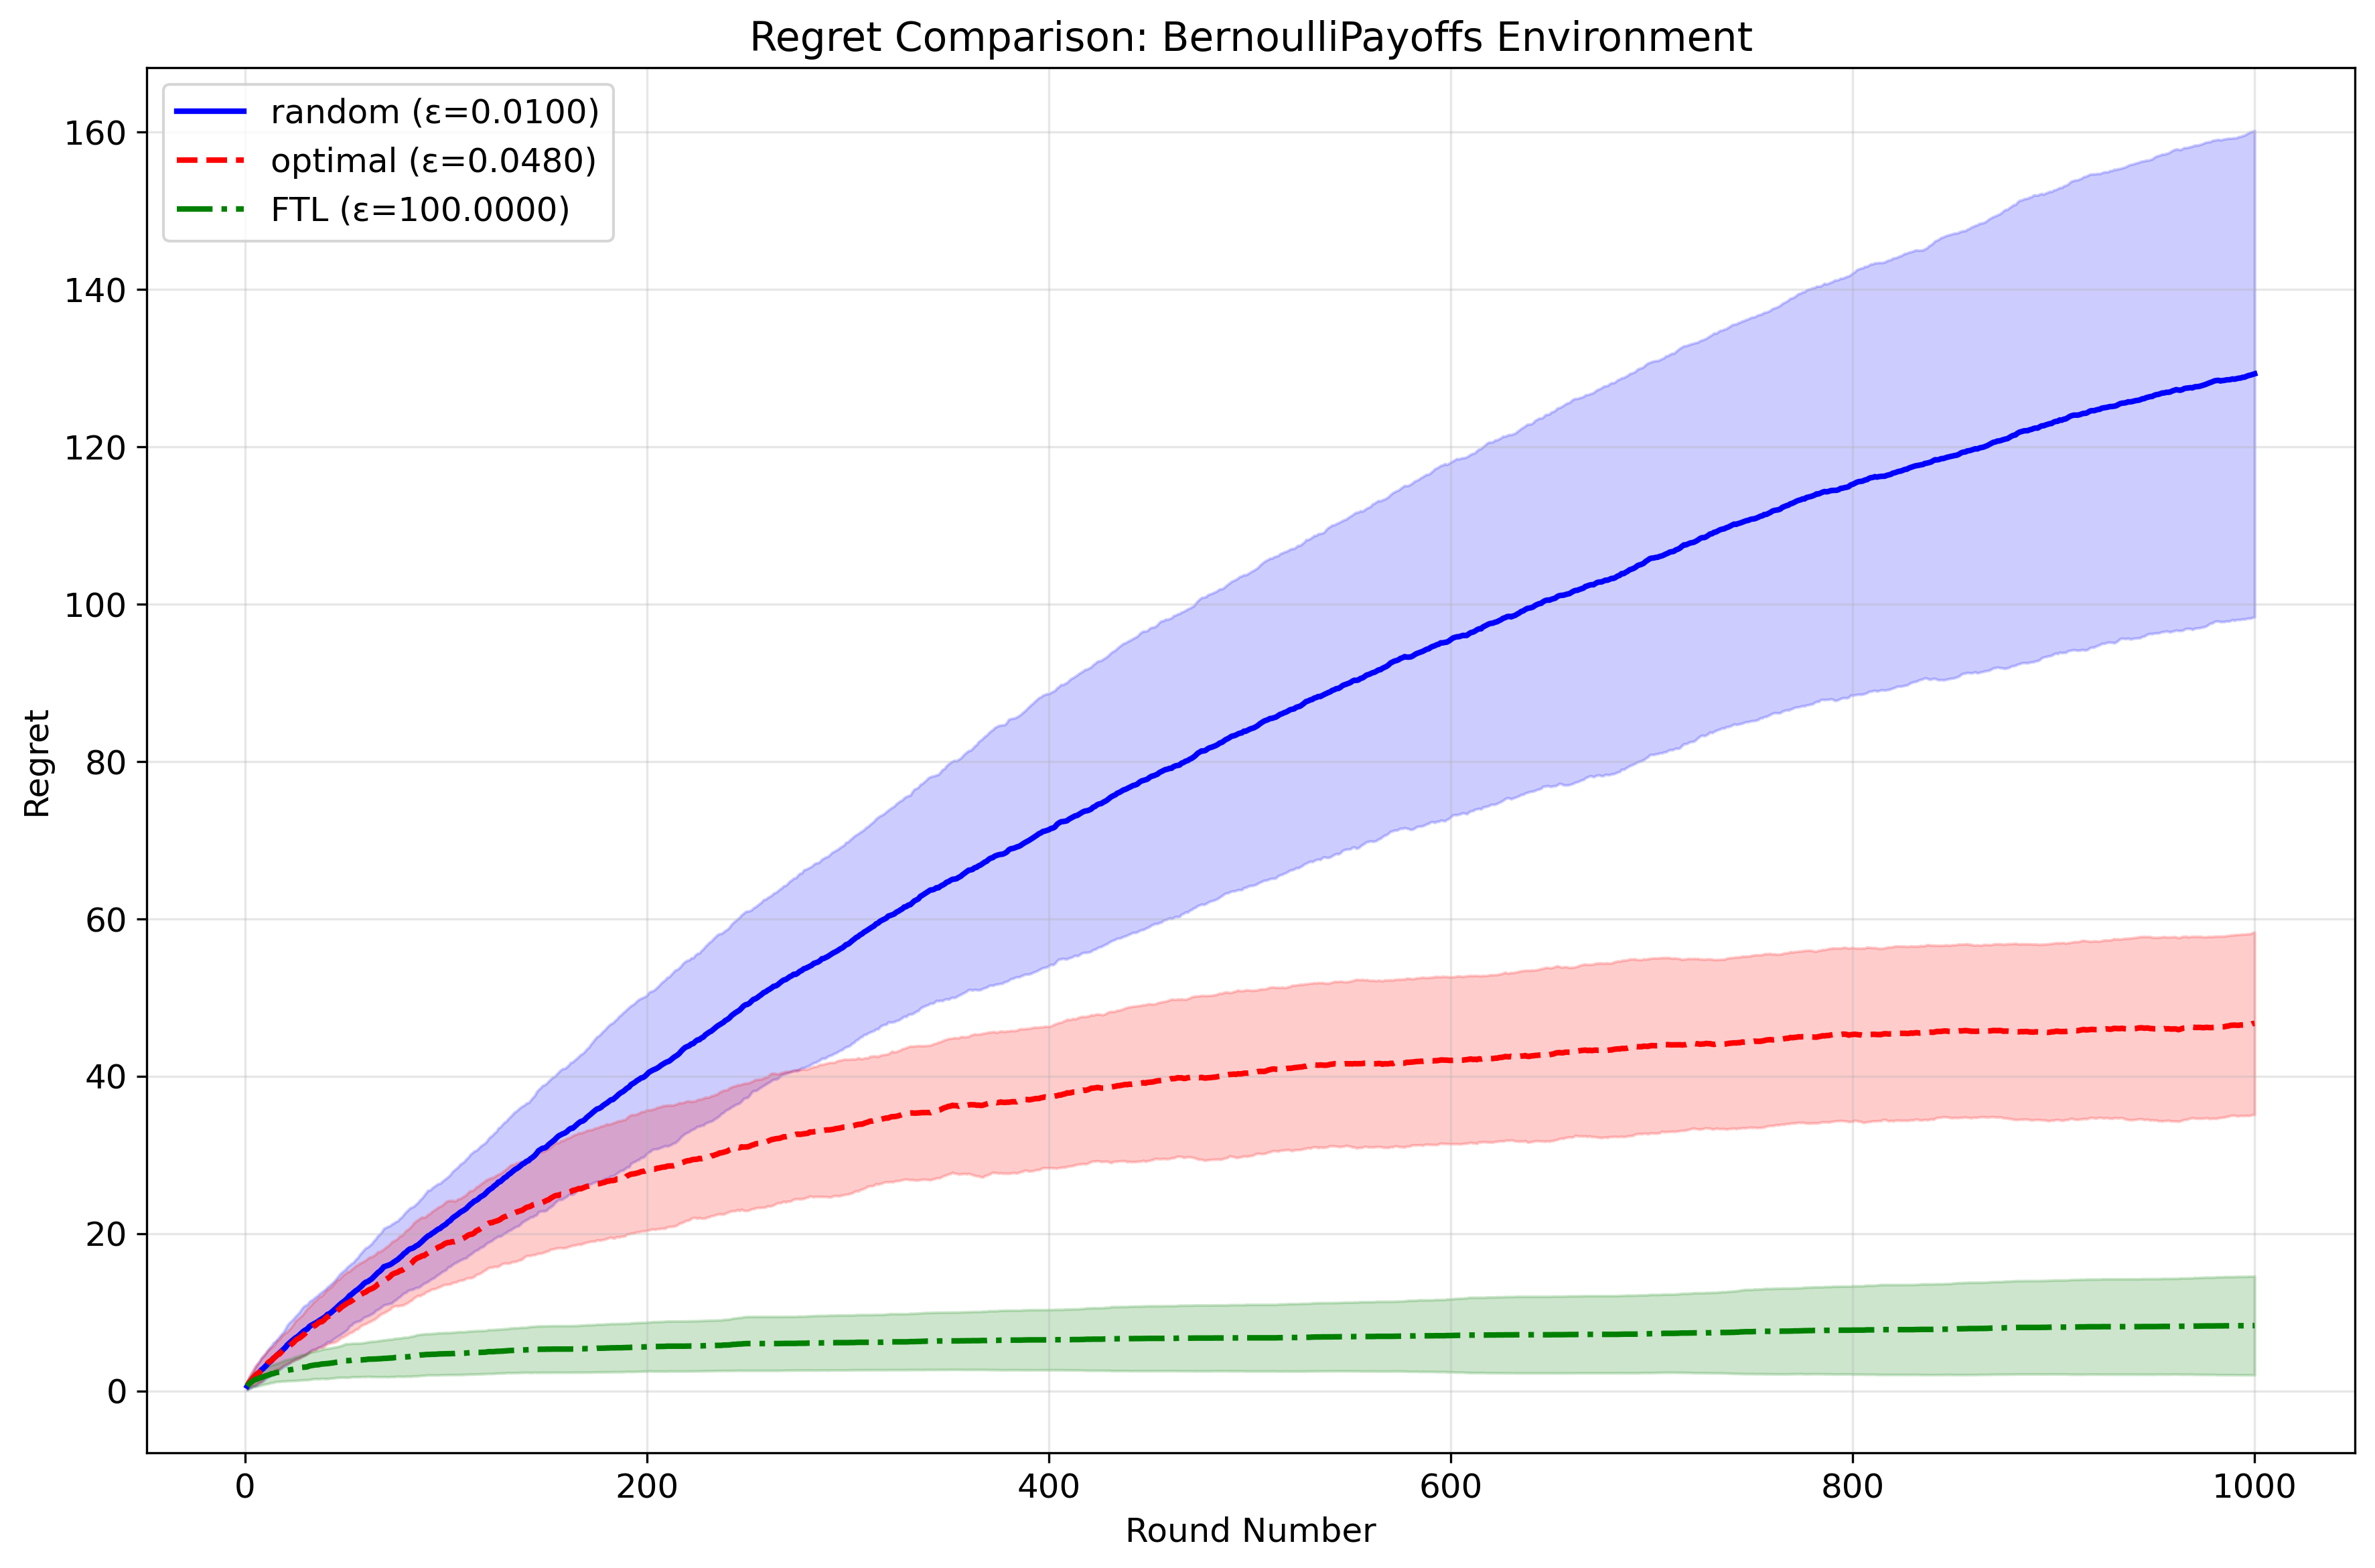
\includegraphics[width=0.5\textwidth]{332Project2/figures/bernoulli_regret_comparison.png}
\end{center}
\end{frame}

\begin{frame}{B - Additional Results}
\textbf{Results}\\
To support our initial intuitive, we get another results about ranking
possibility of local optima.because 95 CI so huge.
\begin{center}
    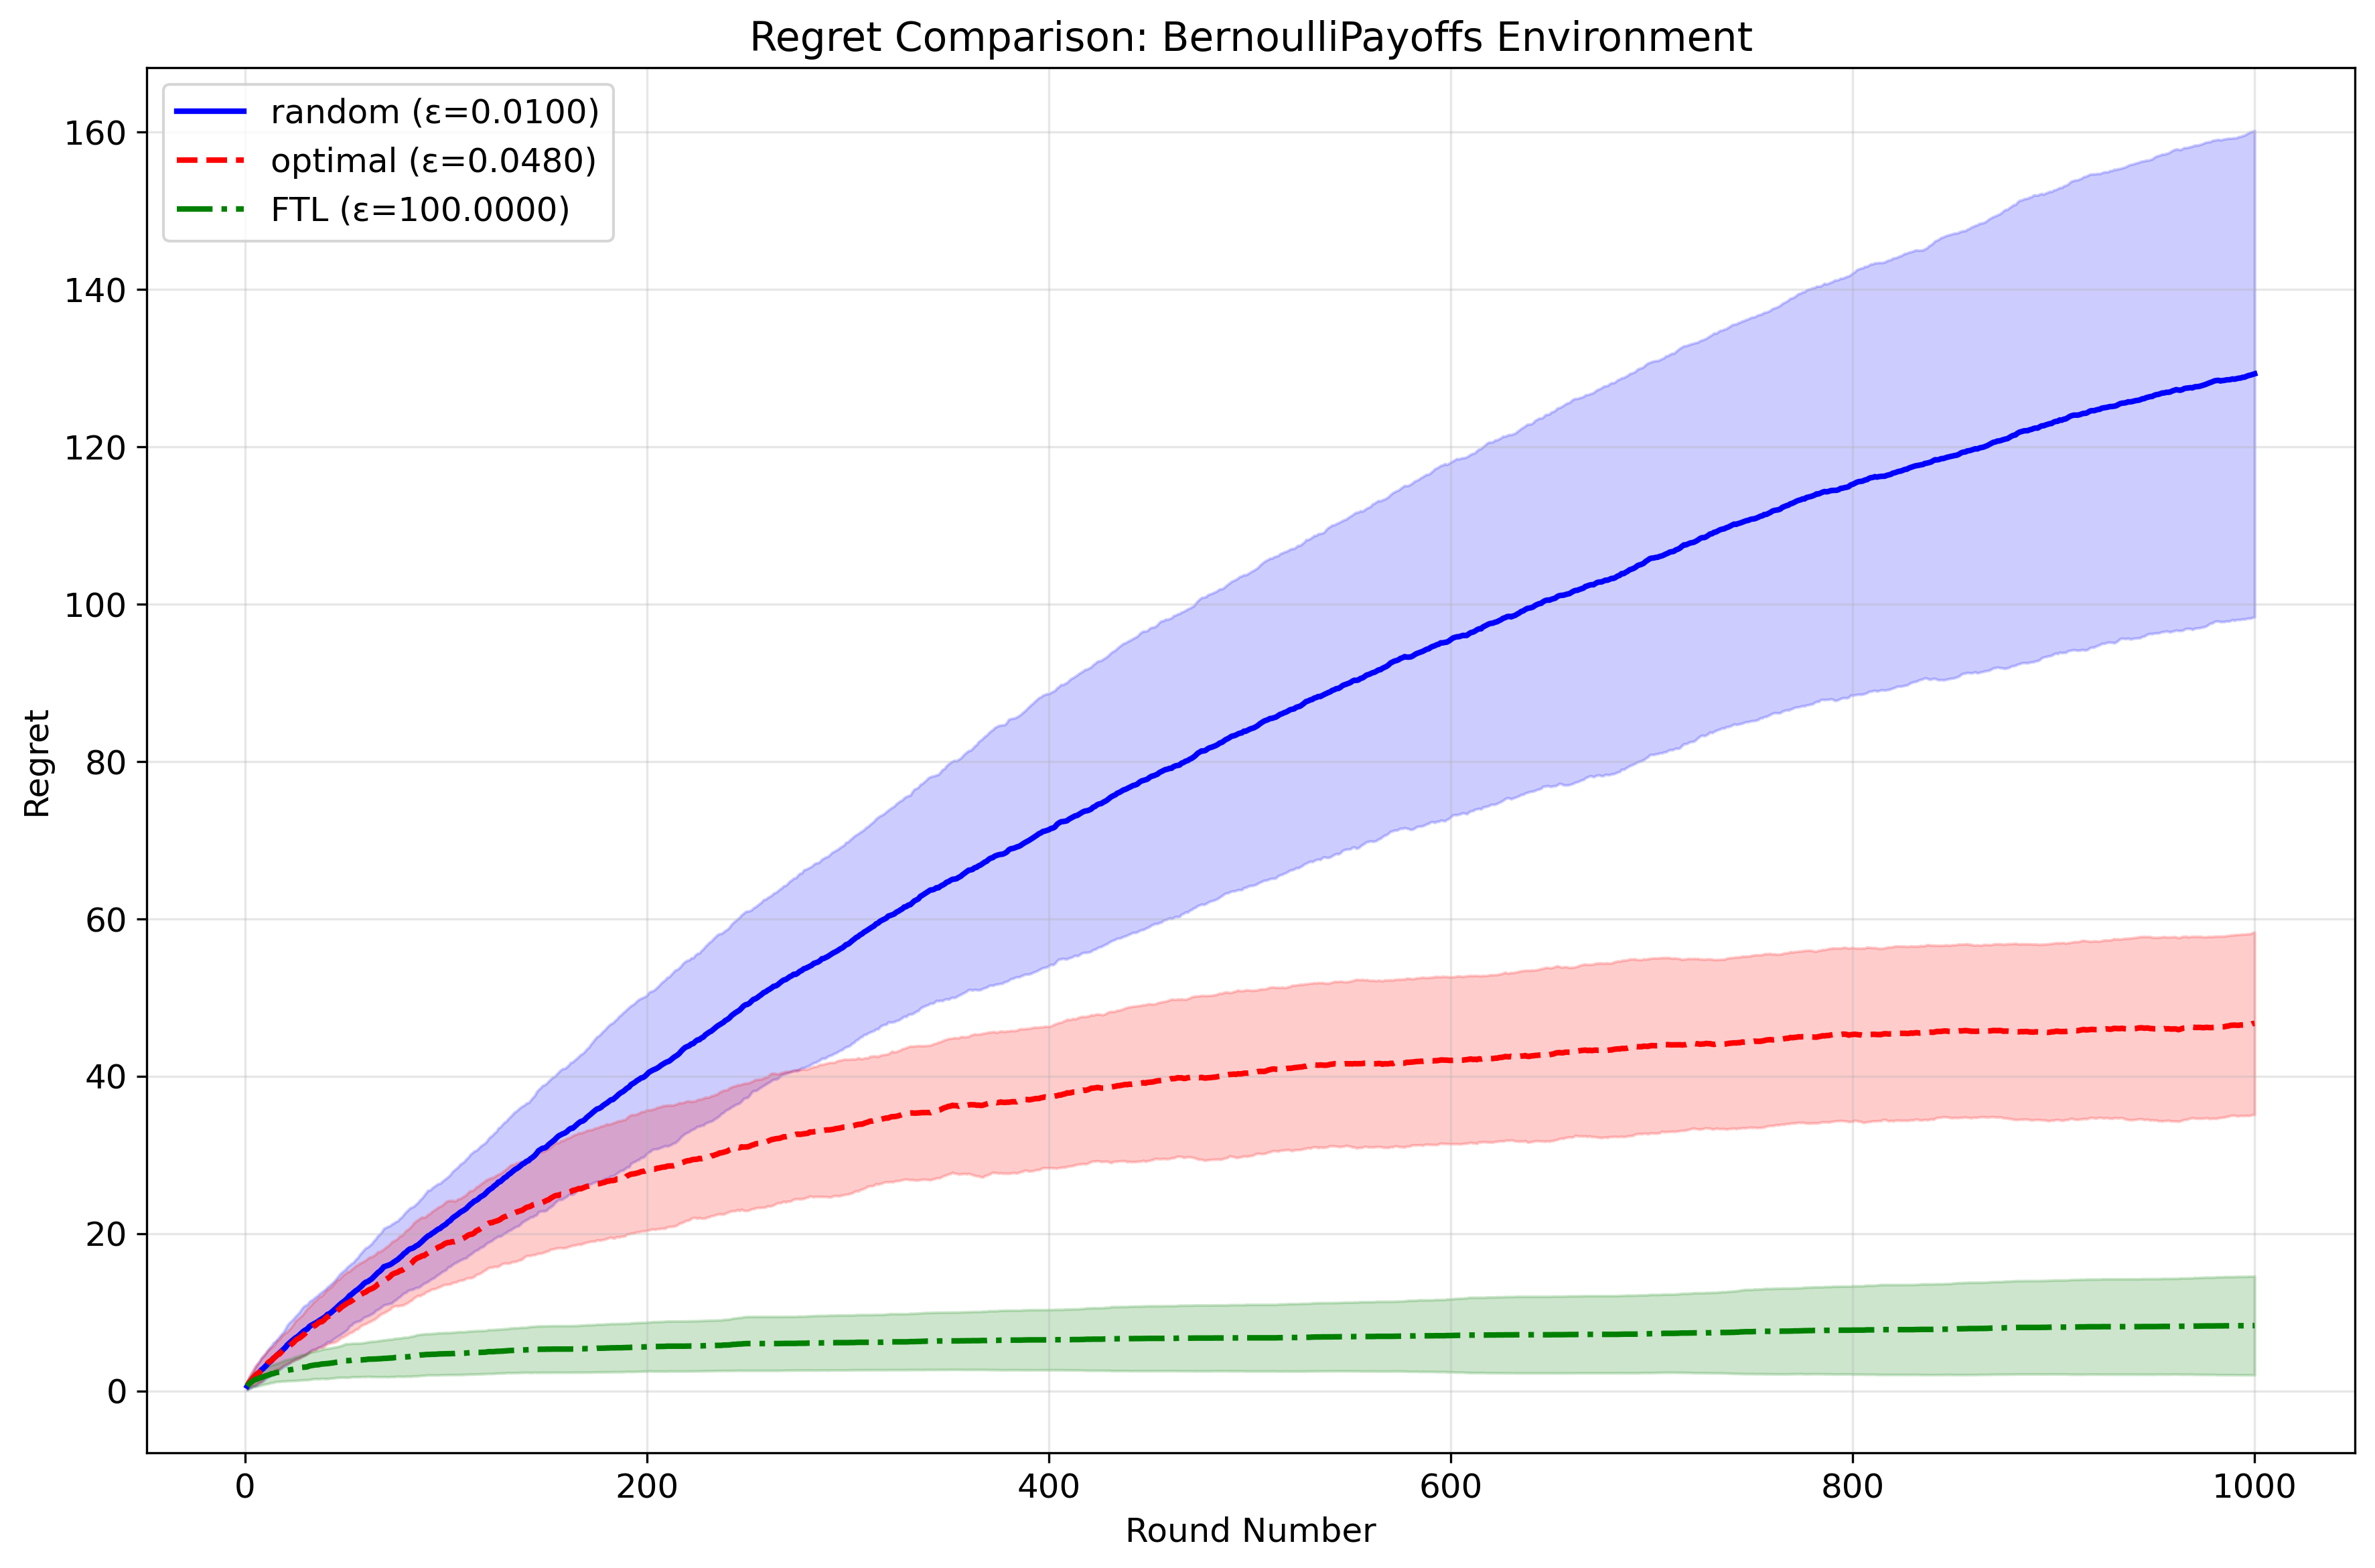
\includegraphics[width=0.5\textwidth]{332Project2/figures/bernoulli_regret_comparison.png}
\end{center}
\end{frame}

\begin{frame}{B - Results(Payoffs)}
\textbf{Results}\\
Calculating regret bound in this setting. it is consistent with result
\begin{center}
    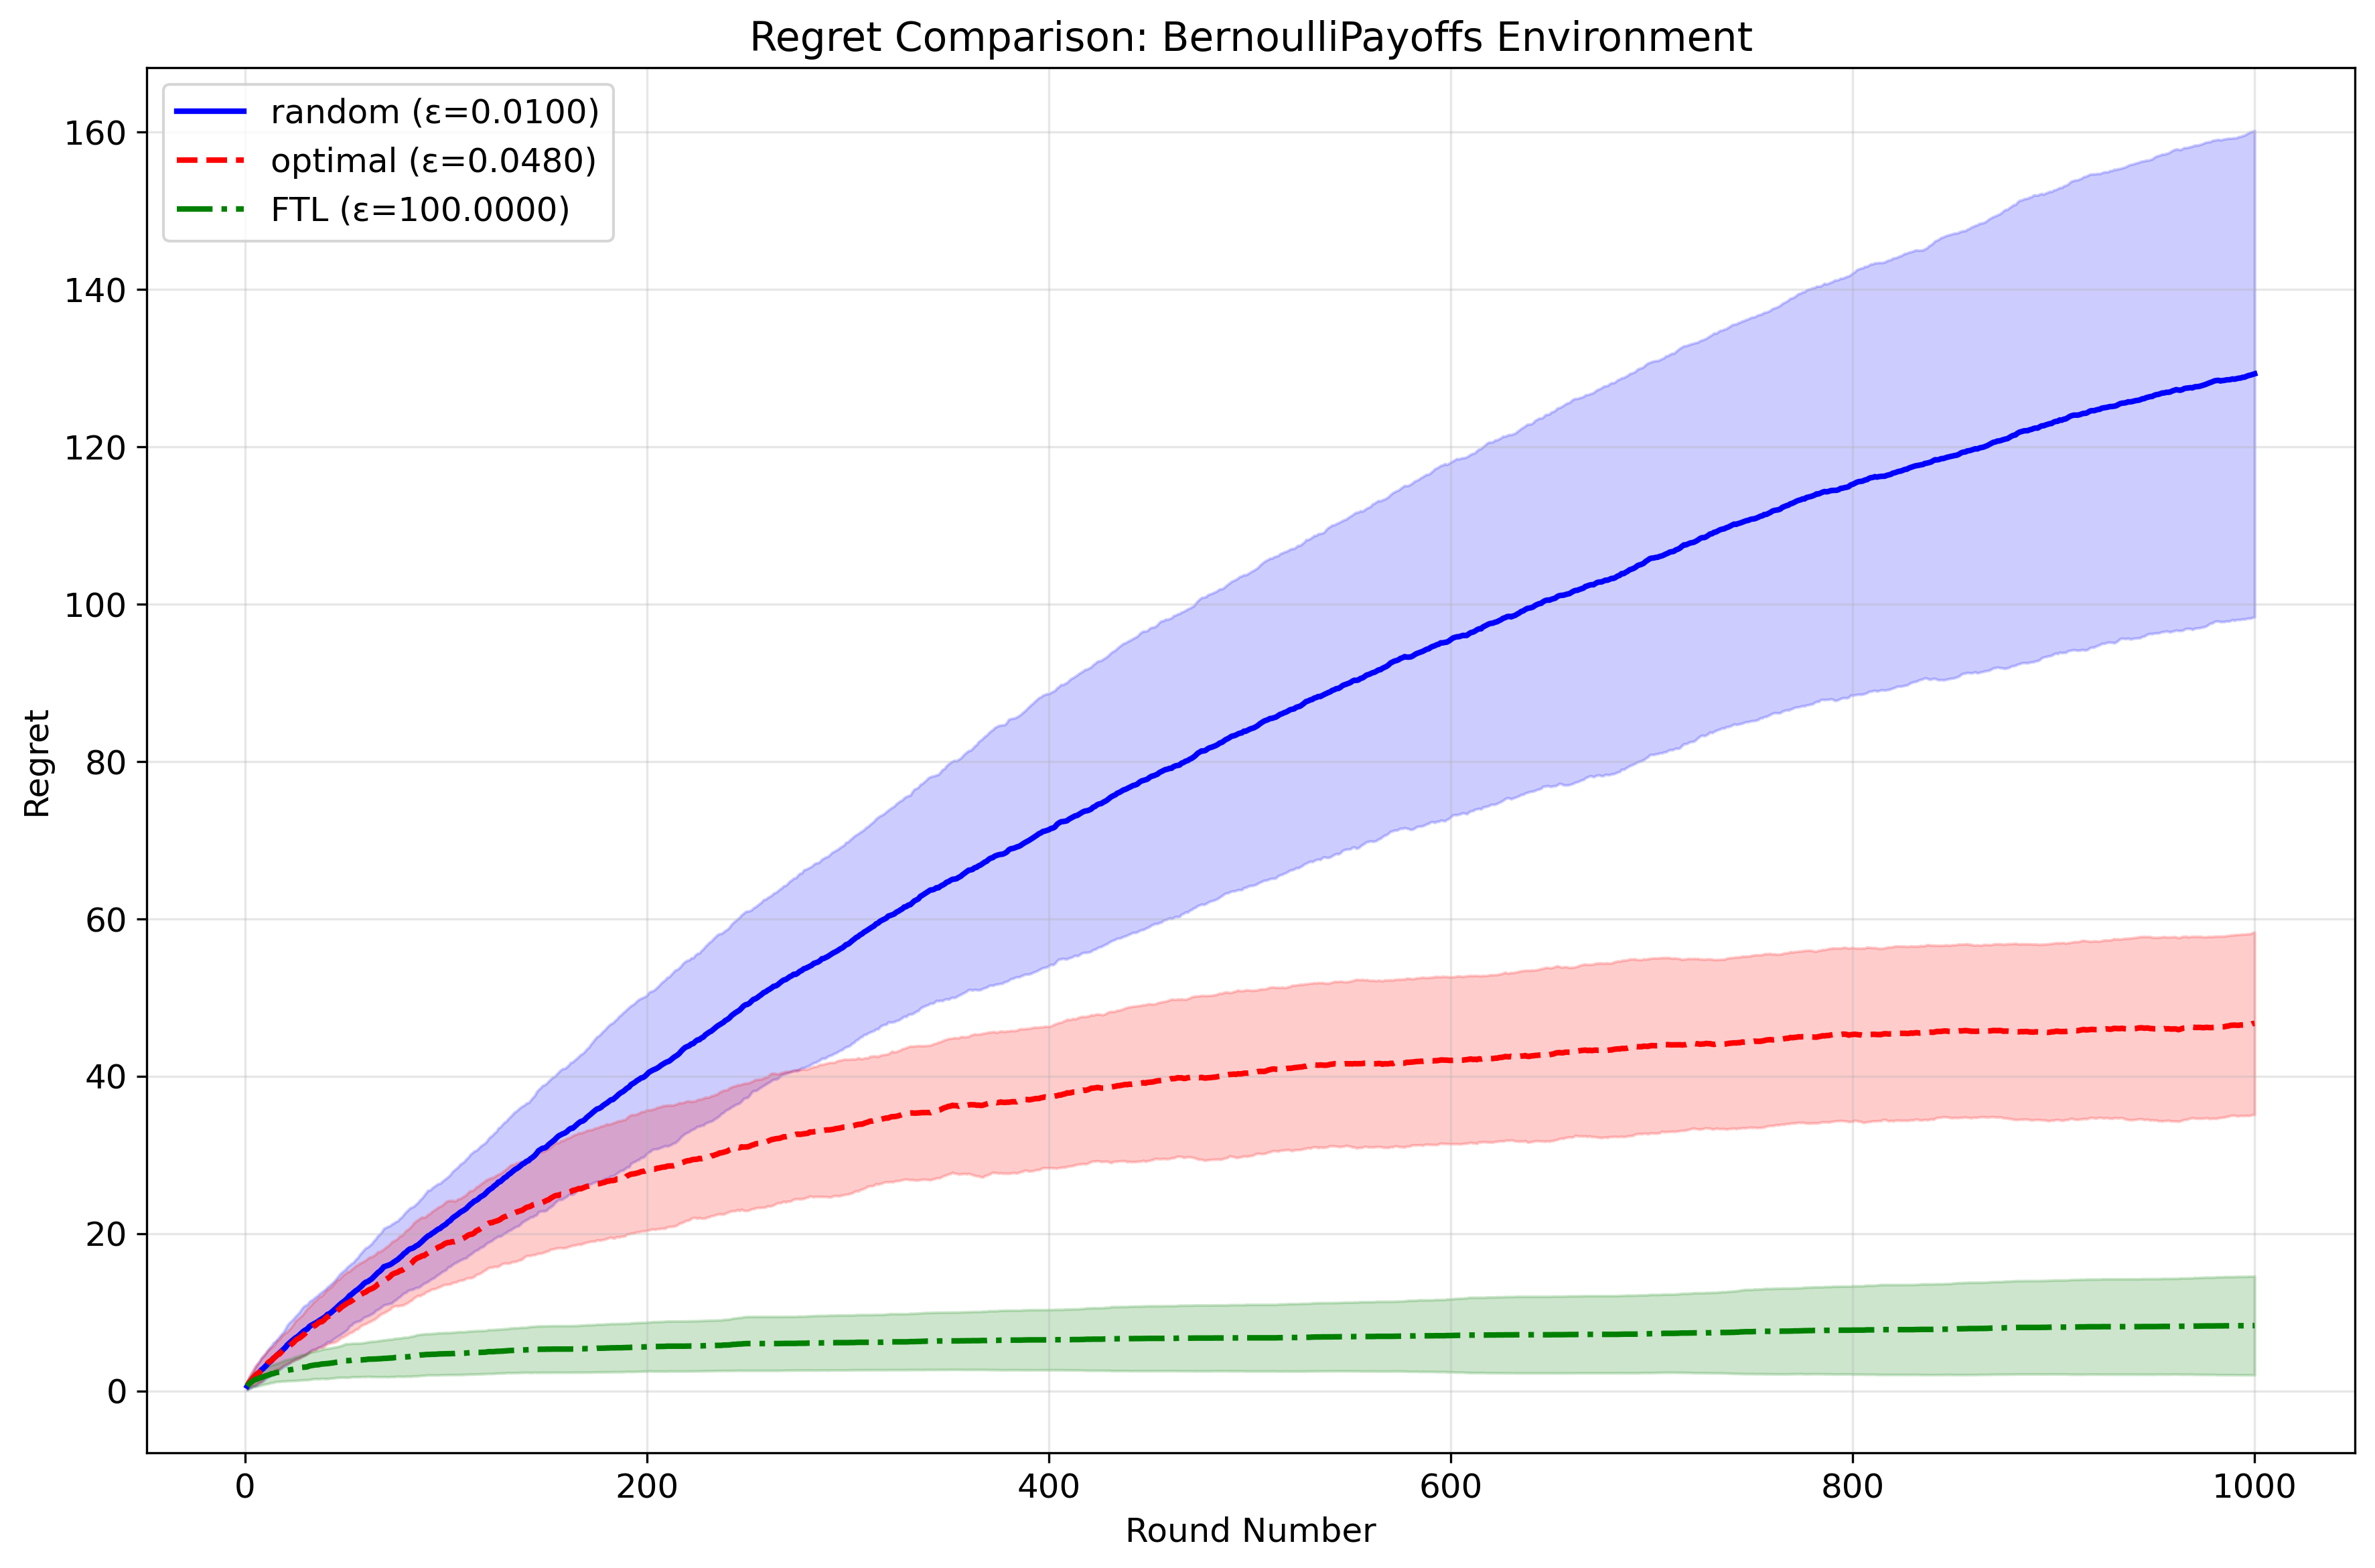
\includegraphics[width=0.5\textwidth]{332Project2/figures/bernoulli_regret_comparison.png}
\end{center}
\end{frame}

\begin{frame}{B - Results(Regret bound)}
\textbf{Results}\\
Calculating regret bound in this setting. it is consistent with result
\begin{center}
    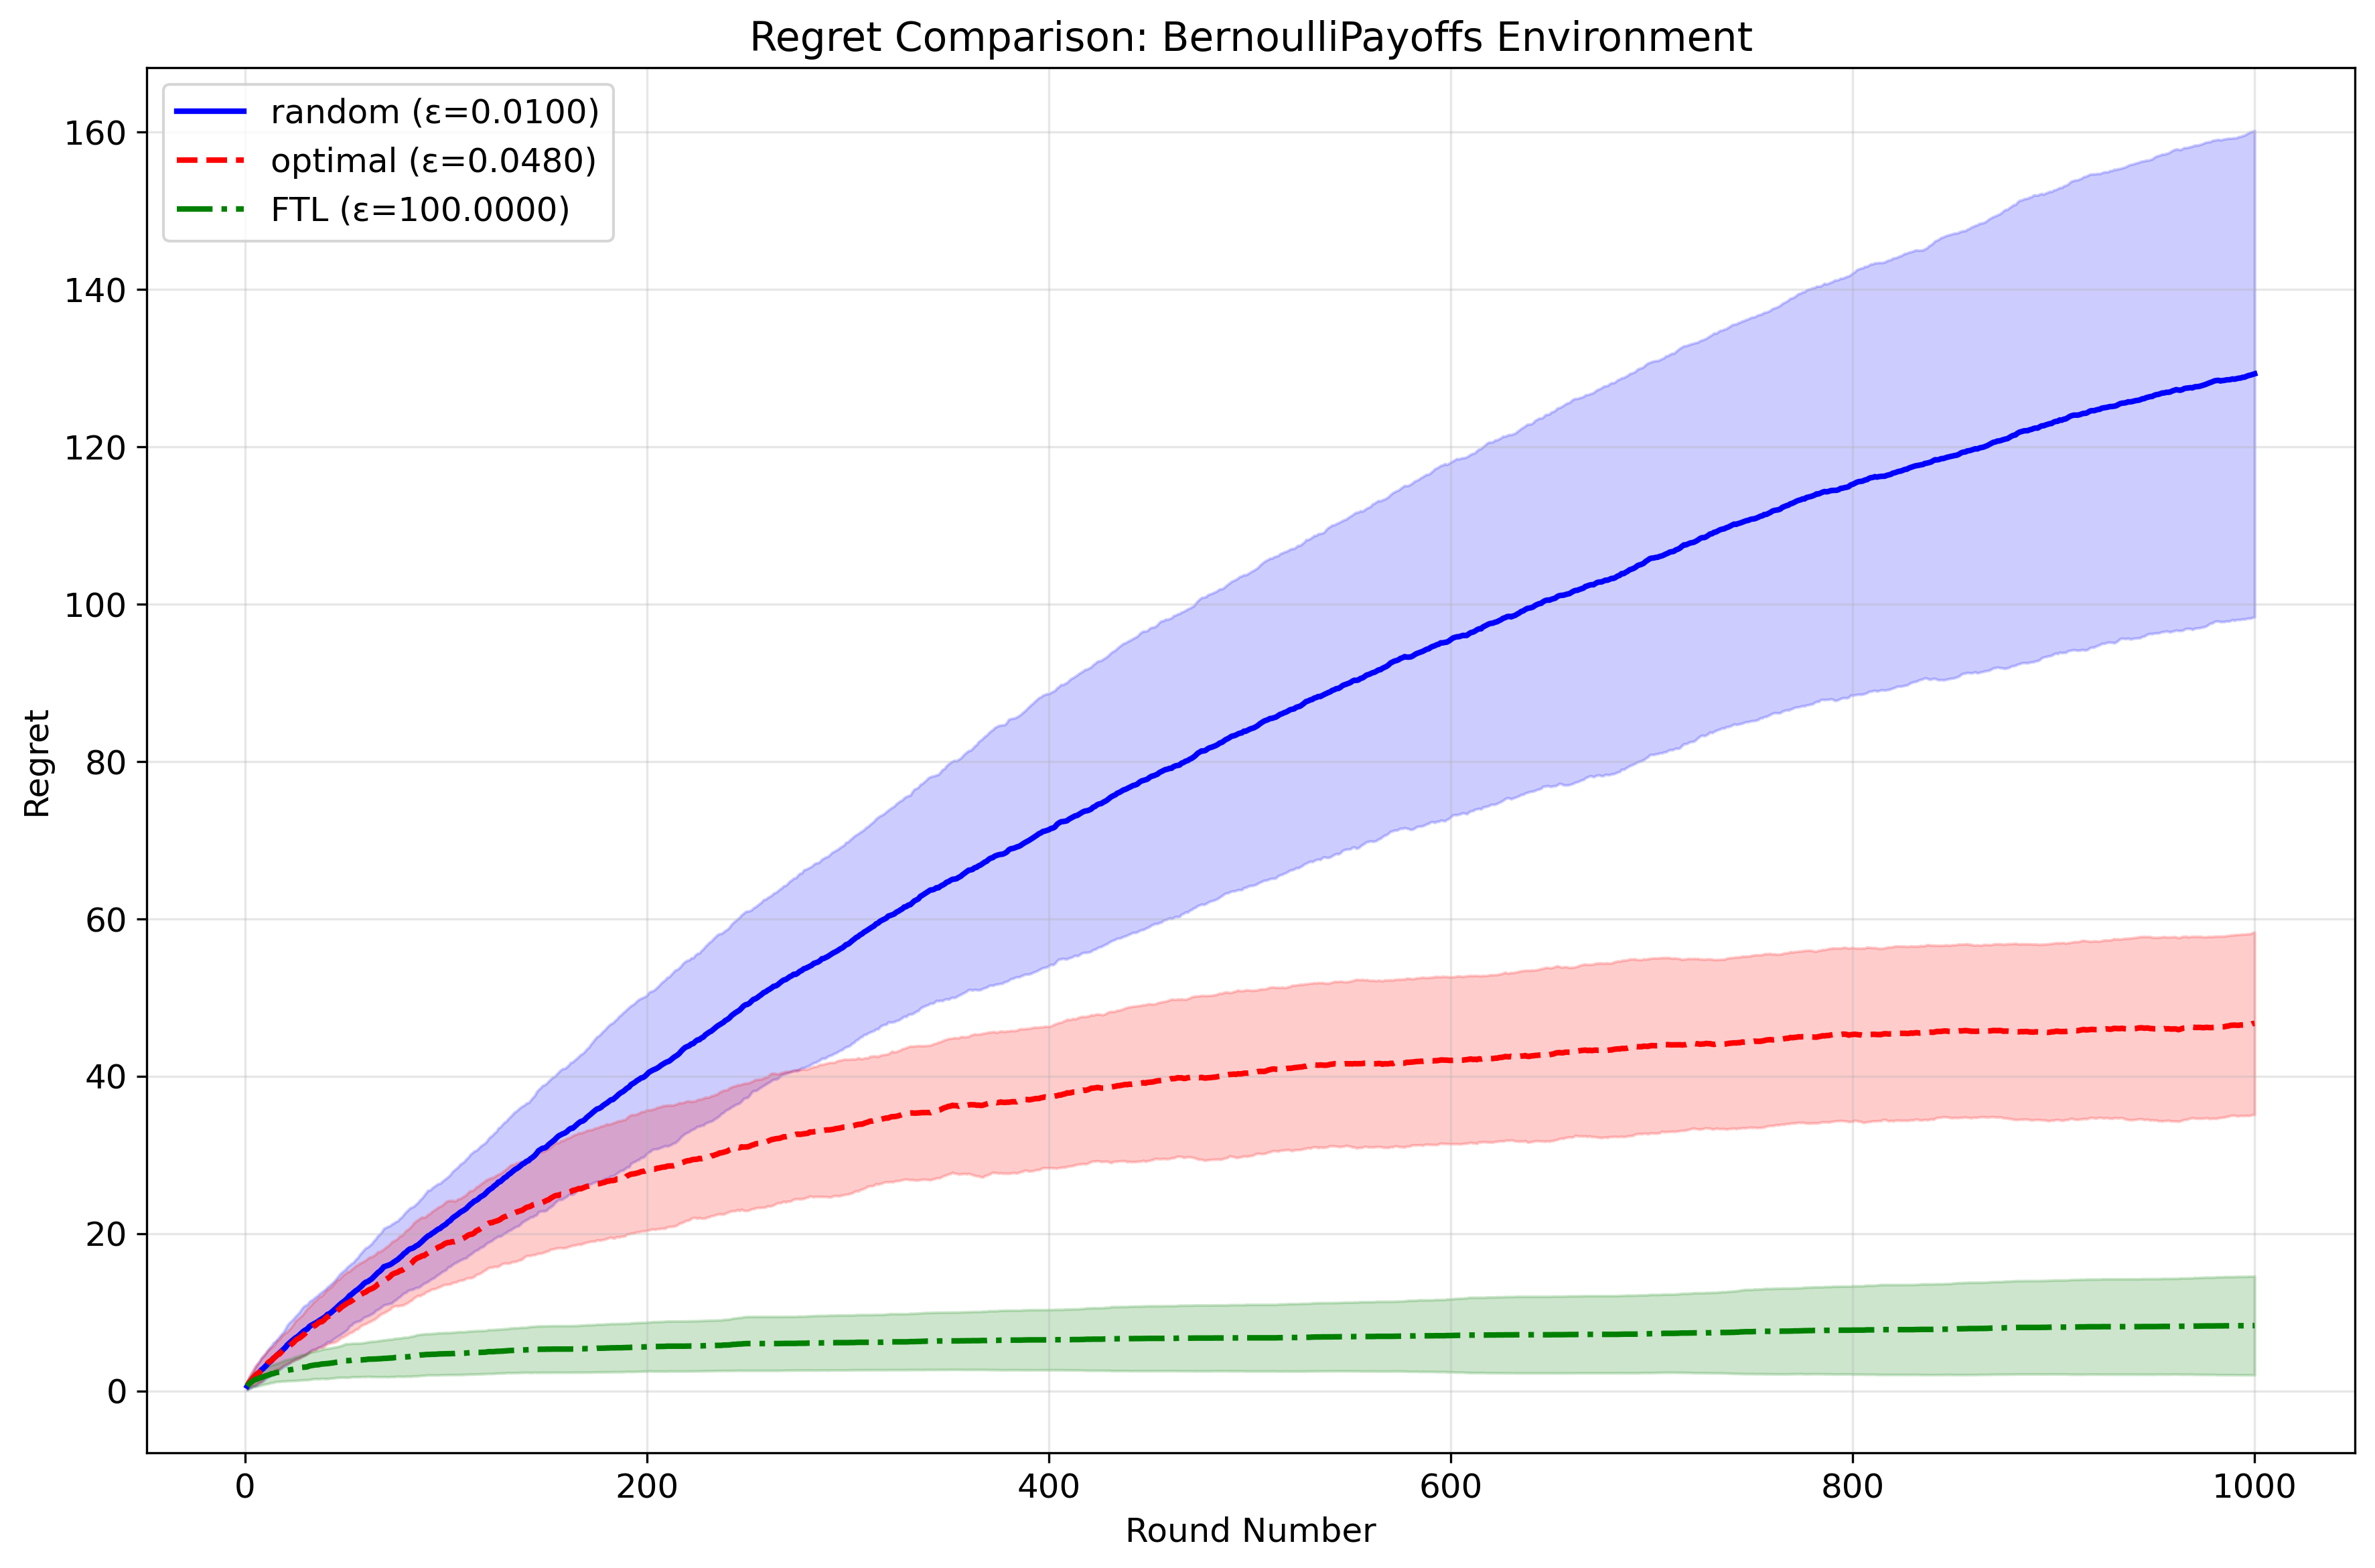
\includegraphics[width=0.5\textwidth]{332Project2/figures/bernoulli_regret_comparison.png}
\end{center}
\end{frame}


\section{Part2}

\begin{frame}{Part2 - Outline}
In Part 2, we consider two things;
\begin{enumerate}
    \item EW algorithm applied to Pachinko Payoffs (PP)
    \item Research Payoffs (RP)
    \begin{itemize}
        \item we modeled our research environment; characterizing research style with AI.
    \end{itemize}
\end{enumerate}
\end{frame}


\begin{frame}{Part2 - Summary}

\textbf{Methods}\\

\textbf{Results}\\

\textbf{Takeaways}\\

\end{frame}

\subsection{C : PP}

\begin{frame}{C - Description of Japanese Pachinko}
In this part, we collect data from Japanese Pachinko (slot machine in Japan).\\
Here's our setting. 

\end{frame}

\begin{frame}{C - Description of Data}
We use data from somewhat trusted data source of pachinko among this community.

\end{frame}

\begin{frame}{C - Setting}
Payoffs are extracted from data

\end{frame}

\begin{frame}{C - Game Structure and Intuition}

\end{frame}

\begin{frame}{C - Results(Regret)}

    
\end{frame}


\begin{frame}{C - Results(Payoffs)}

    
\end{frame}

\begin{frame}{C - Results(Regret bound)}

    
\end{frame}



\subsection{D : RP}
\begin{frame}{D - Setting}
As A and B in this presentation, we fisrt introduce model then show its results.
Here's setting; 

    
\end{frame}

\begin{frame}{D - Game structure and Intuition}
As A and B in this presentation, we fisrt introduce model then show its results.
Here's setting; 

    
\end{frame}

\begin{frame}{D - Results(Regrets)}

    
\end{frame}

\begin{frame}{D - Results(Payoffs)}

    
\end{frame}

\begin{frame}{D - Results(Regret Bound)}

    
\end{frame}

\section{Usage of AI}
\begin{frame}{Usage of AI}
    AI was used for coding, making images;\\
    final review and responsibility by the authors.
\end{frame}

\end{document}